\scanpage{3}
\diagram{\begin{tikzcd}[ampersand replacement=\&,column sep=large,row sep=large]
 \& X_{zar}\arrow[dl]\arrow[dr] \& \\
X_{conn}\arrow[rr,dashed]\arrow[dr,"\text{équiv -- car 0}"]\arrow[dd,"\substack{\text{équiv.}\\\text{si }X/S\text{ lisse}}"'] \& \& X_{\mathbb{P}\text{-}conn.}\arrow[dl,dashed]\arrow[dd,"\substack{\text{équiv}\\\text{si }X/S\text{ lisse}}"]\\
 \& X_{strat}\arrow[dd] \& \\
X_{cris}\arrow[rr,dashed]\arrow[dr]\arrow[dddr] \& \& X_{\mathbb{P}\text{-}cris}\arrow[dl,dashed]\arrow[dddl]\\
 \& X_{inf}\arrow[dd] \& \\
 \& \& \\
 \& X_{zar} \&
\end{tikzcd}}

\margin{$\left.\vphantom{\begin{matrix}X\\X\\X\\X\end{matrix}}\right\}$ morphismes de topos \uline{annelés}
[$\dashrightarrow$ définis si $X$ de torsion sur $\mathbb{Z}$]}

\margin{NB $\mid$ $S$ sous-entendu dans notations.}

Les flèches à valeurs dans $X_{zar}$ donnent lieu à des \uline{isomorphismes de localisation} \uline{\unsure{gerbienne|galoisienne}}, resp. des suites spectrales \unsure{intéressantes} --

\margin{détermination des \uline{points} de ces topos ?}

Les flèches en provenance de $X_{zar}$ donnent lieu à une suite exacte
\[
0\longrightarrow J\longrightarrow\mathcal{O}_{X}\longrightarrow\mathcal{O}_{X_0}\longrightarrow0
\]
\margin{\figure{\begin{tikzpicture}\draw (0,-1.1)--(.65,1.1);\node[anchor=west,text width=4cm] at (.6,0) {dire que $\operatorname{Mod}(X_{zar})\xrightarrow{\approx}\operatorname{Mod}(\mathcal{O}_{X_0})$};\end{tikzpicture}}}

Pour un module inversible $\underline{L}$ sur $X_{zar}$, \unsure{on|--} définit une classe de Chern $c^{\unsure{1|'}}(\underline{L})$ dans $H^2(X_{cris})$ et $H^2(X_{\mathbb{P}\text{-}cris})$, qui sont compatibles si $X$ de torsion. Sur $X_{cris}$, son annulation est NS pour que $\underline{L}$ provienne d'un Module inversible sur $X_{cris}$ [donc dans le cas relatif lisse \deleted{\unsure{disons}} qu'il admette une connexion intégrable].
\mspage{2}
